\chapter{Rozpoznawanie akordów muzycznych}

% wstęp/skrót całego rozdziału
Rozpoznawanie akordów muzycznych zostało zrealizowane za pomocą sieci neuronowych. Wykorzystana
została popularna ostatnio w wielu obszarach architektura transformera
\cite{vaswani_attention_2017}. Modele tego typu były wykorzystywane w najnowszych pracach związanych
z rozpoznawaniem akordów, w tym w pracy \cite{park_bi-directional_2019} stanowiącej główny punkt
odniesienie dla niniejszych badań.

Podczas realizacji zadania rozpoznawania akordów, w pierwszej kolejności zreprodukowane zostały
wyniki z pracy referencyjnej. W tym celu wykonany został zwykły trening nadzorowany, z
wykorzystaniem zbliżonego zbioru danych, zbliżonej procedury i identycznego modelu, jak w
oryginalnych badaniach.

W następnej kolejności model został uproszczony i pozbawiony specjalnych usprawnień, po czym wykonana
została seria eksperymentów, mająca na celu uzyskać tym modelem jak najlepsze wyniki. Celem tego
etapu było przygotowanie punktu odniesienia dla późniejszych eksperymentów z uczeniem
nienadzorowanym. Model został uproszczony, aby nie zaciemniać właściwego tematu pracy, jakim jest
wykorzystanie uczenia nienadzorowanego.

Mając przygotowany działający i stosunkowo prosty model, który uzyskuje wyniki zbliżone do
najlepszych w literaturze, można było przejść do treningów nienadzorowanych, a dokładnie
samonadzorowanych (ang. \emph{self-supervised}). Wykonana została seria czasochłonnych i
zasobożernych eksperymentów, wykorzystujących jedynie dane bez oznaczeń, dzięki którym uzyskano
pretrenowane (ang. \emph{pre-trained}) sieci. Na końcu te pretrenowane modele zostały dotrenowane do
zadania rozpoznawania akordów i wyniki porównano z tymi, uzyskanymi bez uczenia wstępnego.

% co zawiera rozdział
W niniejszym rozdziale opisana została szczegółowo wykorzystana architektura sieci neuronowej.
Następnie przedstawione zostały procedury i zasady treningów nadzorowanego i nienadzorowanego oraz
reguły oceny wytrenowanego modelu. Na końcu opisane zostały wszystkie wykonane eksperymenty i
przeprowadzona została dyskusja otrzymanych wyników.

% model (model.py), trening nadzorowany (training.py), trening nienadzorowany (mae_training.py) i
% ewaluacja (evaluate.py)
\section{Algorytm rozpoznawania akordów muzycznych}

% wstęp - dyskusja na temat podejścia do rozpoznawania akordów (TODO: czy to dobry wstęp i w ogóle
% dobry tytuł tej pierwszej z dwóch części rozdziału, może ta dyskusja powinna być gdzieś indziej)
Jak wspomniano powyżej, do rozpoznawania akordów muzycznych wykorzystano sieci neuronowe. Modele te
są jednak bardzo ogólne i wykorzystując je, wciąż można podejść do zadania rozpoznawania akordów na
bardzo wiele różnych sposobów. Samo zadanie polega właściwie na podzieleniu wejściowego nagrania
muzycznego na logiczne części, w których wybrzmiewają pojedyncze, rozpoznane przez algorytm akordy.
Można więc potraktować to zadanie jako dwa podzadania, albo przeformułować je tak, aby było prostsze
ale dawało takie same rezultaty. 

Po pierwsze należy więc zadać sobie pytanie, z jaką dokładnością mają być rozpoznawane chwile
rozpoczęcia i zakończenia trwania akordów. Sygnał dźwiękowy jest sygnałem ciągłym, ale zapisany jest
w postaci cyfrowej z określoną częstotliwością próbkowania. Można zatem próbować rozpoznawać akordy
z największą możliwą dokładnością, czyli co do pojedynczej próbki. Jest to jednak dokładność
zdecydowanie nadmiarowa w kontekście tego zadania. Zakładając z kolei, że dane wejściowe nie
będą miały postaci surowych próbek ale postać spektrogramu, dokładność rozpoznawania można
ograniczyć do pojedynczych ramek czasowych tworzących spektrogram. Podejście takie jest o tyle
proste, że zadanie rozpoznawania akordów staje się stricte zadaniem klasyfikacji ramek spektrogramu,
które są po prostu wektorami pewnych cech. Uzyskana dokładność czasowa, rzędu dziesiątych części
sekundy, wydaje się być jak najbardziej wystarczająca. Takie też podejście zostało zastosowane w
niniejszej pracy, co jasno widać po opisanym w poprzednim rozdziale wstępnym przetwarzaniu danych.

Kolejnym tematem jest sposób przetwarzania ramek spektrogram przez sieć neuronową. Teoretycznie
każda ramka może być najpierw klasyfikowana osobno, bez uwzględnienia kontekstu przed i po danej
chwili czasu. Powstała w ten sposób, zapewne dość zaszumiona sekwencja akordów, może być wygładzona
kolejnym algorytmem. Wiele podejść tego typu było wcześniej stosowanych. Lepszym pomysłem wydaje się
jednak wykorzystanie szerszego kontekstu czasowego na etapie rozpoznawania pojedynczych akordów.
Można np.  podawać na wejście sieci dłuższy (trwający więcej niż sekundę) fragment a rozpoznawać
jedynie akord brzmiący na samym środku tego fragmentu, jak to zostało zrobione w
\cite{korzeniowski_fully_2016}.  Wciąż można później zaaplikować algorytm uwzględniający szerszy
kontekst, czyli np. konkretne progresje akordów. Najlepiej by jednak było, gdyby model rozpoznający
akordy był jeden i łączył w sobie zarówno informacje lokalne (brzmiące w danym ułamu sekndy
częstotliwości) jak i informacje globalne (progresje akordów). Można więc podawać na wejście sieci
od razu dłuższy fragment utworu i z dokładnością do ramek czasowych dokonywać swego rodzaju
segmentacji semantycznej, czyli przypisywać klasę dla każdej ramki. Takie podejście zostało właśnie
zastosowane w \cite{park_bi-directional_2019}. Idąc za tym najprostszym i być może najbardziej
naturalnym pomysłem zastosowano go również w niniejszej pracy. 

\subsection{Opis wykorzystanego modelu sieci neuronowej}

Do rozpoznawani akordów, podobnie jak w \cite{park_bi-directional_2019}, wykorzystany został
popularny w ostatnim latach model sieci neuronowej, o nazwie \emph{Transformer}. W niniejszej pracy,
poza fazą reprodukcją wyników z \cite{park_bi-directional_2019}, wykorzystana została jak
najprostsza i jak najbardziej zbliżona do oryginału wersja tego modelu. Implementacja została,
przygotowana samodzielnie (plik \url{src/training/model.py}) na bazie literatury i innych
implementacji.

\subsubsection{Krótka historia transformerów}

% krótka historia transformera (TODO: czy to do przeglądu literatury czy tutaj)
Model transformera został oryginalnie wprowadzony jako model do przetwarzania języka naturalnego, w
pracy \cite{vaswani_attention_2017}. Była to architektura typu \emph{enkoder-dekoder}, służąca np.
do tłumacznie z jednego języka na drugi. Wcześniej do zadań związanych z językiem naturalnym były
głównie wykorzystywane sieci rekurencyjne, które miały problem, aby dobrze radzić sobie z długimi
sekwencjami słów --- zapominały kontekst jeżeli przetwarzany tekst nie był dość krótki. W celu
rozwiązania tego problemu wprowadzono mechanizm atencji (ang. \emph{attention}), który pozwalał
uwzględnić dalszy kontekst zdania \cite{bahdanau_neural_2016}. Pomysł twórców transformera polega na
tym, aby zrezygnować z sieci rekurencyjnych i pozostawić jedynie mechanizm atencji, w połączeniu z
warstwami liniowymi i funkcjami aktywacji (MLP). Transformer nie jest więc ani siecią rekurencyjną,
ani siecią splotową. Po odniesieniu ogromnego sukcesu w NLP (dziś praktycznie wszystkie modele do
NLP są budowane na bazie transformerów), architektura ta została wykorzystana również w
przetwarzaniu obrazów \cite{dosovitskiy_image_2021}. Na potrzeby klasyfikacji zdjęć została nieco
uproszczona ponieważ pozostawiony został sam enkoder. Na tym polu transformery również odniosły
sukces, chociaż nie wyparły sieci splotowych \cite{liu_convnet_2022}, tak jak wyparły sieci
rekurencyjne. Ostatecznie modele tego typu zostały wykorzystane również do przetwarzania dźwięku, w
tym do klasyfikacji dźwięków \cite{gong_ast_2021} i do rozpoznawania mowy
\cite{kim_squeezeformer_2022}. Transformery są więc dziś bardzo popularnymi modelami, które znajdują
zastosowanie praktycznie w każdej dziedzinie, wykorzystującej uczenie maszynowe.

\subsubsection{Ogólny opis architektury}

\begin{figure}
    \centering
    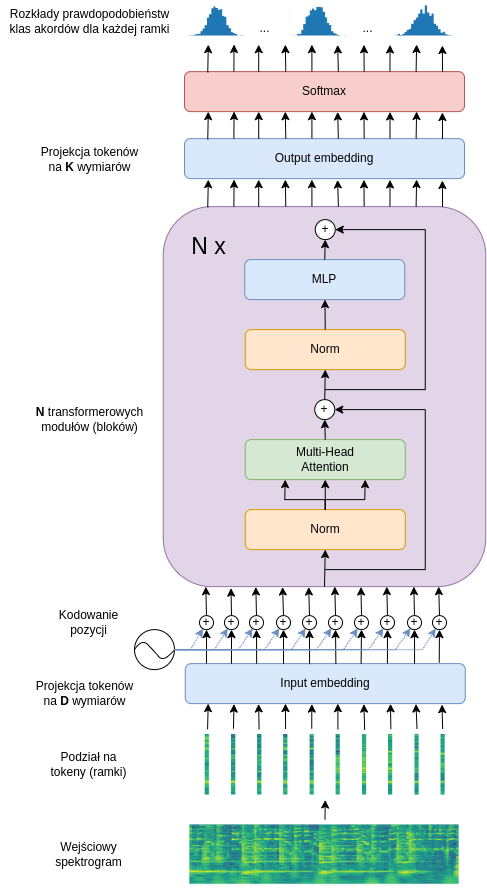
\includegraphics[width=0.8\textwidth]{./images/transformer.png}
    \caption{Schemat modelu transformera do rozpoznawania akordów muzycznych}
    \label{fig:transformer}
\end{figure}

% ogólny opis architektury - wejście
Rysunek \ref{fig:transformer} prezentuje wykorzystany do treningów model sieci neuronowej ---
transformer. Architektura tego modelu jest bardzo prosta. Na wejście sieci podawany jest składający
się z $N$ ramek spektrogram $\defmatrix{S}{N}{F}$, który następnie dzielony jest (tylko ideowo, w
praktyce to wciąż pojedyncza macierz) na ramki (wektory $\vec s_i \in \mathbb{R}^F$). Ramki pełnią
rolę tokenów, czyli np. kolejnych słów w przypadku przetwarzania języka naturalnego. Transformer
przetwarza cały ciąg tokenów równolegle, co jest jego podstawową przewagą nad sieciami
rekurencyjnymi, które przetwarzają ciąg tokenów w sposób sekwencyjny. W praktyce jednocześnie przez
sieć może przejść kilka ciągów tokenów, czyli cały \emph{batch} sekwencji. Długość sekwencji tokenów
jest zupełnie arbitralna, ten sam model może przetwarzać sekwencje różnej długości, zarówno w
treningu jak i później, podczas inferencji.

% ogólny opis architektury - input embedding i positional encodding
W pierwszej kolejności sekwencja ramek (macierz $\matrix{S}$) przechodzi przez pojedynczą warstwę
liniową, która rzutuje tokeny wejściowe na wybraną dla danego modelu liczbę wymiarów
$d_{\mathrm{model}}$:
\begin{equation}
    \matrix{T_{in}} = \matrix{S} \matrix{W_{in}}
\end{equation}
gdzie $\defmatrix{T_{in}}{N}{d_{\mathrm{model}}}$ to wyjściowa macierz tokenów a
$\defmatrix{W_{in}}{F}{d_{\mathrm{model}}}$ to macierz parametrów tej warstwy. Liczba wymiarów
$d_{\mathrm{model}}$, podobnie jak liczba tokenów $N$, nie zmienia się podczas przechodzenia przez
kolejne warstwy, co różni transformer od sieci splotowych, gdzie rozmiar danych przechodzących przez
sieć jest sukcesywnie zmniejszany. W rzeczywistości istnieją architektury oparte o oryginalny
transformer, które podobnie jak sieć splotowa, zmniejszają rozmiar danych wejściowych
\cite{liu_swin_2021}, ale to tylko głupie wymysły Microsoftu. Przed wejściem do stanowiących
właściwą część transformera serii bloków, do tokenów dokładana jest informacja o ich pozycji w
sekwencji --- jest to kodowanie pozycji (ang. \emph{positional encoding}). Szczegóły tej operacji
zostały opisane poniżej.

% ogólny opis architektury - bloki, w tym MLP i normalizacja
Centralną część transformera stanowi ciąg identycznych bloków BLK. Liczba tych bloków ($B$), w
połączeniu z wymiarowością tokenów ($d_{\mathrm{model}}$), stanowią główne hiperparametry modelu i
decydują o jego rozmiarze. Każdy blok składa się z dwóch głównych warstw: warstwy atencyjnej MSA
(ang. \emph{Mulit-Head Self-Attention}) i niewielkiego perceptrona wielowarstwowego MLP (ang.
\emph{Mulitlayer Perceptron}). Każdą z tych warstw poprzedza normalizacja Norm typu \emph{Layer
Normalization} \cite{ba_layer_2016}, a kończy połączenie rezydualne \cite{he_deep_2015}, czyli
dodanie do wartości na wyjściu nieznormalizowanej wartości z wejścia. Operacje realizowane przez
pojedynczy blok dla ciągu tokenów $\defmatrix{T}{N}{d_{\mathrm{model}}}$ można opisać równaniami:
\begin{eqnarray}
     \textrm{MSA}'(\matrix{T}) = \textrm{MSA}(\textrm{Norm}(\matrix{T})) + \matrix{T} \\
     \textrm{MLP}'(\matrix{T}) = \textrm{MLP}(\textrm{Norm}(\matrix{T})) + \matrix{T} \\
     \textrm{BLK}(\matrix{T}) = \textrm{MLP}'(\textrm{MSA}'(\matrix{T}))
\end{eqnarray}
Zastosowana nomalizacja aplikowana jest niezależnie (choć równolegle) dla każdego tokena $t \in
\mathbb{R}^{d_{\mathrm{model}}}$ z sekwencji $\matrix{T}$. Polega ona na odjęciu wartości średniej
tokena oraz podzieleniu przez jego odchylenie standardowe. Przedstawia to wzór:
\begin{equation}
    \textrm{Norm}(t) = \frac{t - \textrm{E}[t]}{\sqrt \textrm{Var}[t]} \cdot \gamma + \beta
\end{equation}
gdzie $\gamma$ i $\beta$ to trenowane parametry warstwy, przesuwające i skalujące odpowiednio wynik
normalizacji. Jeżeli chodzi o perceptron wielowarstwowy, to ma ona zawsze dwie warstwy ukryte, z
wymiarem ukrytym czterokrotnie większym niż $d_{\mathrm{model}}$ oraz funkcją aktywacji GELU.
\begin{equation}
    \textrm{MLP}(\matrix{T}) = \textrm{GELU}(\matrix{T}\matrix{W_1} + b_1)\matrix{W_2} + b_2
\end{equation}
gdzie wejściem jest sekwencja tokenów $\defmatrix{T}{N}{d_{\mathrm{model}}}$, macierze
$\defmatrix{W_1}{d_{\mathrm{model}}}{4d_{\mathrm{model}}}$,
$\defmatrix{W_2}{4d_{\mathrm{model}}}{d_{\mathrm{model}}}$ oraz wektory (dodawane do każdego wiersza
odpowiedniej macierzy) $b_1 \in \mathbb{R}^{4d_{\mathrm{model}}}$ i $b_2 \in
\mathbb{R}^{d_{\mathrm{model}}}$ to parametry dwóch warstw ukrytych perceptrona wielowarstwowego.

% ogólny opis architetury - dropout
W rzeczywistości pojedynczy blok zawiera jeszcze jeden opcjonalny element, jakim są warstwy
\emph{dropout}, umieszczone w trzech miejscach: po funkcji aktywacji w module MLP oraz po każdym z
dwóch połączeń rezydualnych, czyli w połowie bloku i na jego wyjściu. Dodatkowo \emph{dropout} może
być stosowany również przed wejściem do sieci, czyli bezpośrednio na spektrogramie. Warstwy tego
typu zerują z wybranym prawdopodobieństwem niektóre z przechodzących przez nie wartości w celu
regularyzacji sieci i uniknięcia przetrenowania. Technika ta jest opcjonalna i nie była stosowana we
wszystkich eksperymentach.

% ogólny opis architektury - wyjście (klasyfikacja)
Po serii bloków następuje ostatnia część modelu, odpowiedzialna za klasyfikację. Najpierw,
utrzymywana przez wszystkie bloki, wymiarowość tokenów jest zmieniana przez warstwę liniową, w
zależności od liczby klas $K$.
\begin{equation}
    \matrix{T_{out}} = \matrix{T} \matrix{W_{out}}
\end{equation}
gdzie $\defmatrix{T_{out}}{N}{K}$ to macierz wyjściowa, $\defmatrix{T}{N}{d_{\mathrm{model}}}$ to
macierz sekwencji tokenów a $\defmatrix{W_{out}}{d_{\mathrm{model}}}{K}$ to macierz parametrów tej
warstwy liniowej. Następnie dla każdego tokena $t \in \mathbb{R}^K$ zwracany jest rozkład
prawdopodobieństwa przynależności do poszczególnych klas akordów, za pomocą funkcji \emph{softmax}:
\begin{equation}
    \textrm{softmax}(t_i) = \frac{\exp{t_i}}{\sum_{j=1}^{K}\exp{t_j}}
\end{equation}
gdzie $t_i$ to $i$-ty element wektora (tokena) $t$. Podsumowując, na wejściu sieci jest spektrogram,
składający się z $N$ ramek i $F$ cech, a na wyjściu jest $N$ rozkładów prawdopodobieństwa między $K$
klas, dla każdej z ramek spektrogramu. Wszystkie ramki spektrogramu są więc klasyfikowane
jednocześnie, ale z uwzględnieniem kontekstu, jaki tworzą razem.

\subsubsection{Kodowanie pozycji tokenów}

% positional encoding
Jak widać na rysunku \ref{fig:transformer}, pomiędzy projekcją tokenów wejściowych a wejściem do
serii bloków, jest jeszcze etap kodowania pozycji każdego z tokenów. Etap ten jest niezbędny aby
zawrzeć w każdym z tokenów informację o tym, jaka jest jego pozycja w sekwencji. W przypadku sieci
rekurencyjnych, informacja ta jest zawarta niejawnie, poprzez przetwarzanie tokenów jeden po drugim,
w odpowiedniej kolejności. W przypadku transformerów, gdzie tokeny są przetwarzane równolegle,
informacja ta musi być dodana jawnie.  Istnieje wiele sposobów, według których można zakodować
pozycję tokenów, głównie dzielących się na wykorzystanie wartości wyuczonych (parametry modelu) i
stałych (odpowiednia funkcja).  W niniejszej pracy wykorzystane zostało podejście oryginalnych
twórców transformera, oparte o wartości funkcji sinus i kosinus. Polega ono na tym, że dla każdego
tokena (dla każdej pozycji) generuje się wektor, który ma tę samą liczbę wymiarów co token, dzięki
czemu może być do niego dodany. Wartości tych wektorów zdefinowane są wzorami:
\begin{equation}
    PE_{(\textrm{pos},2i)} = \sin(\textrm{pos}/10000^{2i/d_{\textrm{\tiny model}}})
\end{equation}
\begin{equation}
PE_{(\textrm{pos},2i + 1)} = \cos(\textrm{pos}/10000^{2i/d_{\textrm{\tiny model}}})
\end{equation}
Równania te oznaczają, że każdy wymiar wektora kodującego pozycję odpowiada sinusoidzie o innej
częstotliwości. Parzyste pozycje w wektorze to wartości odpowiednich funkcji sinus dla danej
pozycji, a nieparzyste to wartości funkcji kosinus dla danej pozycji. Stosowany jest również
wariant, gdzie pierwsza połowa wektora to wartości funkcji sinus a druga to wartości funkcji
kosinus. Autorzy uzasadniają, że użycie tych funkcji pozwala modelowi łatwo wykorzystywać informację
o pozycji, ponieważ między wektorami prezentującymi różne pozycje występują zależności liniowe. Na
rysunku \ref{fig:positional_encoding} przedstawiono graficzną reprezentację wektorów kodujących
pozycję, dla sekwencji składającej się ze 100 tokenów (wiersze), gdzie liczba wymiarów każdego z
nich to 256 (kolumny).
\begin{figure}
    \centering
    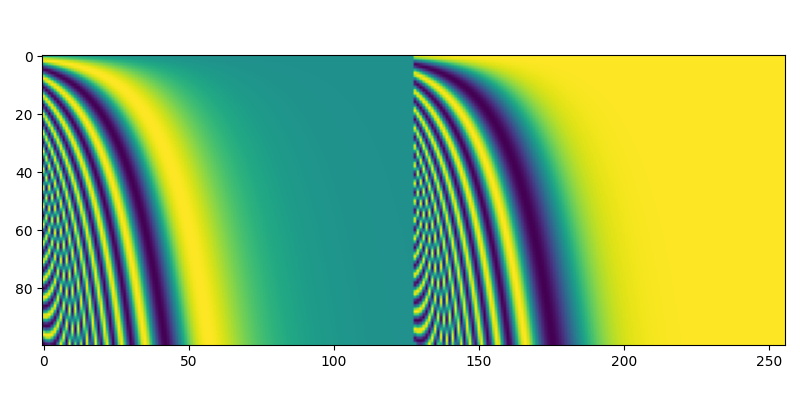
\includegraphics[width=1.0\textwidth]{./images/positional_encoding.png}
    \caption{Przykład wektorów kodujących pozycję dla sekwencji 100 tokenów o wymiarowości 256}
    \label{fig:positional_encoding}
\end{figure}

\subsubsection{Multi-Head Self-Attention}

% mutli-head self-attention - wstęp
Najważniejszą część transformera stanowi warstwa atencyjna MSA. Jako jedyna w całym modelu
odpowiada ona za ,,wymianę'' informacji między tokenami --- uwzględnienie kontekstu pozostałych
tokenów w sekwencji, podczas tworzenia nowej reprezentacji danego tokena.

% mutli-head self-attention - ogólnie o mechaniźmie attention
Sama idea mechanizmu \emph{Attention} polega na tym, że mając dla danego tokena wejściowego
zapytanie (ang. \emph{query}) i mając zbiór par klucz-wartość (ang. \emph{key-value}) związanych z
innym (lub tym samym) ciągiem tokenów, wylicza się nową reprezentację tokena jako ważoną sumę tych
wartości, gdzie wagi są wyliczane na podstawie dopasowania zapytania do kluczy. Wagi te informują
więc o tym, jak dużo uwagi powinno poświęcić się danej wartości, tworząc nową reprezentację danego
tokena. W przypadku zadania tłumaczenia maszynowego, mechanizm ten pozwala skupić się na
odpowiednich częściach sekwencji wejściowej, podczas tworzenia sekwencji wyjściowej. Jeżeli zarówno
zapytania jak i pary klucz-wartość pochodzą z tej samej sekwencji tokenów, mamy do czynienia z
\emph{Self-Attention}. Warstwa tego typu wyznacza więc dla każdego tokena w sekwencji zapytanie,
klucz i wartość, a następnie tworzy jego nową reprezentację jako ważoną sumę wartości pozostałych
tokenów. Informacje zakodowane w poszczególnych tokenach mieszają się zatem między sobą. W praktyce
warstwa atencyjna w transformerze realizuje równolegle kilka niezależnych operacji
\emph{Self-Attention}, których wyniki na końcu są łączone w całość, stąd też nazwa \emph{Multi-Head
Self-Attention}. Pozwala to uzyskać lepsze rezultaty niż pojedyncza operacja, nawet jeżeli
wykorzysta się niżej wymiarowe reprezentacje.

% mutli-head self-attention - dokładnie jak działa, wzorki
Na wejściu warstwy atencyjnej w transformerze znajduje się macierz
$\defmatrix{T}{N}{d_{\mathrm{model}}}$, czyli sekwencja $N$ tokenów. Dla każdego z nich, za pomocą
zwykłych warstw liniowych, wylicza się $H$-krotnie trzy wektory: zapytanie $q_i \in
\mathbb{R}^{d_k}$, klucz $k_i \in \mathbb{R}^{d_k}$ oraz wartość $v_i \in \mathbb{R}^{d_v}$, gdzie
$i \in [1, H]$. Dla całej sekwencji tokenów wektory te tworzą macierze $\defmatrix{Q_i}{N}{d_k}$,
$\defmatrix{K_i}{N}{d_k}$ oraz $\defmatrix{V_i}{N}{d_v}$. Przedstawiają to równania:
\begin{eqnarray}
    \matrix{Q_i} = \matrix{T} \matrix{W_i^Q} \\\
    \matrix{K_i} = \matrix{T} \matrix{W_i^K} \\\
    \matrix{V_i} = \matrix{T} \matrix{W_i^V} \\\
\end{eqnarray}
gdzie macierze $\defmatrix{W_i^Q}{d_{\mathrm{model}}}{d_k}$,
$\defmatrix{W_i^K}{d_{\mathrm{model}}}{d_k}$ oraz $\defmatrix{W_i^V}{d_{\mathrm{model}}}{d_v}$ to
macierze parametrów warstw liniowych tworzących $i$-tą trójkę: zapytanie, klucz i wartość.

Dla pojedynczej trójki macierzy $\matrix{Q}$, $\matrix{K}$ i $\matrix{V}$, operacja
\emph{Self-Attention} wygląda następująco:
\begin{equation} \label{eq:sa}
    \textrm{SA}(\matrix{Q}, \matrix{K}, \matrix{V}) = \textrm{softmax}(\frac{\matrix{Q}\matrix{K^T}}{\sqrt{d_k}})\matrix{V}
\end{equation}
Człon ,,$\textrm{softmax}(\frac{\matrix{Q}\matrix{K^T}}{\sqrt{d_k}})$'' oznacza wyliczenie macierzy
atencji między wszystkimi parami klucz-zapytanie, poprzez wykonanie iloczynów skalarnych dla
każdej z tych par, przeskalowanie uzyskanych wartości i wykorzystanie normalizującej funkcji
\emph{softmax}. Dlatego też funkcja SA nazywa się właściwie \emph{Scaled Dot-Product Attention}.
Wartości w uzyskanej macierzy atencji pełnią rolę wag, które następnie są użyte do stworzenia
nowej reprezentacji wszystkich tokenów, za pomocą średniej ważonej wektorów z macierzy $\matrix{V}$.
Wynik operacji SA jest więc macierzą, o wymiarach $N \times d_v$.

Cała opracja \emph{Multi-Head Self-Attention} polega na $H$-krotnym wykonaniu operacji
\emph{Self-Attention}, których wektory wynikowe są łączone i ostatecznie rzutowane z powrotem na
$d_{\mathrm{model}}$ wymiarów. Przedstawiają to poniższe wzory:
\begin{equation}
    \textrm{MSA}(\matrix{T}) = \textrm{Concat}(\textrm{SA}(\matrix{Q_1}, \matrix{K_1}, \matrix{V_1}), ..., \textrm{SA}(\matrix{Q_H},
    \matrix{K_H}, \matrix{V_H}))\matrix{W^O}
\end{equation}
gdzie macierz $\defmatrix{W^O}{Hd_v}{d_{\mathrm{model}}}$ to parametry ostatniej w ramach bloku
atencyjnego warstwy liniowej, która rzutuje sklejone wektory z pojedynczych operacji SA na
początkowe $d_{\mathrm{model}}$ wymiarów. Dzięki temu wymiarowość tokenów na wyjściu z warstwy
atencyjnej pozostaje taka sama jak na wejściu. W niniejszej pracy zastosowane zostało powszechne
podejście, aby liczbę wymiarów wektorów zapytań, kluczy i wartości ustalić z góry i uzależnić od
liczby wymiarów tokenów i liczby równoległych operacji SA. Zależność ta jest następująca:
\begin{equation}
    d_k = d_v = \frac{d_{\mathrm{model}}}{H}
\end{equation}
Poza wspomnianymi wcześniej hiperparametrami $B$ i $d_{\mathrm{model}}$ istotna dla funkcjonowania
modelu jest również liczba $H$ równoległych operacji SA, nazywana również ,,liczbą głów''. Wszystkie
hiperparametry transformera zostały zebrane w tabeli \ref{tab:transformer_params}.

\begin{table}
    \centering
    \caption{Hiperparametry transformera}
    \label{tab:transformer_params}
    \begin{tabular}{|c|l|} \hline
        Symbol & Znaczenie \\ \hline
        $F$ & Wymiarowość na wejściu \\
        $d_{\mathrm{model}}$ & Wymiarowość tokenów wewnątrz sieci \\
        $B$ & Liczba bloków transformera \\
        $H$ & Liczba ,,głów'' w bloku MSA \\
        $K$ & Liczba klas na wyjściu \\
        $p_d$ & Prawdopodobieństwo warstw \emph{dropout} \\ \hline
    \end{tabular}
\end{table}

\subsubsection{Dwukierunkowy transformer do rozpoznawania akordów --- BTC}

W pracy referencyjnej \cite{park_bi-directional_2019} autorzy postanowili wprowadzić drobne
modyfikacje w stosunku do oryginalnego bloku transformera tworząc swój autorski model nazwany
\emph{bi-directional transformer for chord recognition} (BTC). Pierwszą z nich jest zamiana warstw
liniowych w module MLP, na jednowymiarowe warstwy splotowe z polem recepcyjnym szerokości 3 tokenów.
Według autorów ma to ułatwić sieci tworzenie bardziej ,,wygładzonych'' predykcji i lepsze
wykorzystanie kontekstu otaczającego każdą ramkę. Druga różnica polega na tym, że pojedynczy blok
transformerowy został rozbity na dwa, które dostają te same wartości na wejściu, a ich wartości
wyjściowe są łączone za pomocą dodatkowej warstwy liniowej. Bloki te różnią się operacją MSA.
Została w nich zastosowana technika maskowania, polegająca na modyfikacji macierzy atencji (wzór
\ref{eq:sa}) w ten sposób, że dla danego tokena, wagi wszystkich wcześniejszych lub późniejszych
tokenów są zerowane. Oznacza to, że tworząc nową reprezentację danego tokena wykorzystuje
się jedynie tokeny poprzedzające, lub następujące po nim. W modelu BTC, każdy z dwóch bloków
tworzących moduł MSA ma inny kierunek maskowania. Technika ta ma zmusić model do pełnego
wykorzystywania zarówno wcześniejszego jak i późniejszego kontekstu przy klasyfikacji danej ramki.

\subsection{Procedura treningu nadzorowanego}

% wstęp
Pierwszy z dwóch rodzajów wykonywanych treningów sieci to klasyczny trening nadzorowany.
Wykorzystywane są w nim dane z oznaczeniami aby nauczyć model rozwiązywania konkretnego problemu ---
klasyfikacji akordów muzycznych. 

% zbiory i epoki
Pojedynczy trening nadzorowany (pojedynczy eksperyment) to jednokrotne nauczenie sieci na wszystkich
dostępnych (lub tylko na wybranych podzbiorach --- parametr \emph{subset} w indeksie), oznaczonych
przykładach uczących i ocena wyników wytrenowanego modelu. W eksperymencie zawsze wykorzystywane są
wszystkie trzy części zbioru danych: część treningowa, walidacyjna i testowa. Treningowa służy do
właściwej nauki i optymalizacji parametrów modelu. Zbiór walidacjny wykorzystuje się do sprawdzania
w trakcie nauki, jak model radzi sobie z przykładami, na których nie był uczony (np. czy się
przetrenowuje).  Zbiór testowy wykorzystywany jest po zakończeniu procesu nauki, aby uzyskać
ostateczną ocenę jakości wytrenowanego modelu. Trening dzieli się na epoki, które z definicji
oznaczają pojedyncze przejście przez wszystkie dostępne dane treningowe. Jak opisano w rozdziale
\ref{sec:preprocessing}, w przypadku przeprowadzonych eksperymentów, pojedyncza epoka oznacza
kilkukrotne przejście przez wszystkie utwory treningowe, ale dla każdego utworu przetwarzany jest
jedynie jego losowy fragment (lub fragmenty).

% kroki
Na epokę składają się kroki, gdzie każdy krok oznacza jedną zmianę parametrów modelu. W ramach
każdego kroku model przetwarza równolegle cały \emph{batch} 10-sekundowych fragmentów utworów.
Ponieważ, ze względów optymalizacyjnych, na jeden przykład ze zbioru danych składa się kilka
fragmentów tego samego utworu, to na realny rozmiar batcha wpływają dwa parametry: liczba
analizowanych równolegle przykładów (czyli utworów) oraz liczba zwracanych jednocześnie fragmentów
pojedynczego utworu. Dla każdej ramki, z każdego fragmentu wejściowego, model zwraca predykcję akordów, w
postaci rozkładów prawdopodobieństw. Rozkłady te są następnie porównywane z rzeczywistymi klasami
akordów za pomocą funkcji kosztu, jaką jest entropia krzyżowa (ang. \emph{cross-entropy}). Dla
pojedynczej ramki, czyli dla pojedynczego wyjściowego rozkładu prawdopodobieństw $t \in
\mathbb{R}^K$ i indeksu $k$, oznaczającego numer rzeczywistej klasy tej ramki, entropia krzyżowa ma
postać:
\begin{equation}
    \textrm{CE}(t, k) = - \log t_k
\end{equation}
Wartość tę uśrednia się później między wszystkimi tokenami (ramkami) i między sekwencjami
(fragmentami), aby uzyskać pojedynczą liczbę rzeczywistą, reprezentującą błąd popełniany przez sieć.
Następnie, zgodnie z algorytmem \emph{backpropagation}, obliczane są pochodne cząstkowe (gradient)
tej funkcji kosztu po wszystkich parametrach modelu. Do optymalizacji parametrów modelu na podstawie
obliczonych pochodnych wykorzystany jest algorytm optymalizacyjny \emph{AdamW}. Współczynnik nauki
(ang. \emph{learning rate}), przez pierwszych pięć epok ma jedynie dziesiątą część swojej docelowej
wartości, aby zapewnić małe zmiany parametrów modelu na początku treningu. Transformery są bowiem
podantne na to, że z powodu zbyt dużych kroków w początkowej fazie treningu, przestaną zbiegać do
konkretnego rozwiązania. Dodatkowo, na potrzeby późniejszej analizy, w każdym kroku zapisywane są
wartości funkcji kosztu i metryki \emph{accuracy} dla obecnego batcha przykładów.

% walidacja
Pod koniec każdej epoki, po przejściu przez cały zbiór treningowy, następuje bieżąca ocena modelu na
zbiorze walidacyjnym. Aby zapewnić stabilność wyników tej oceny, nie stosuje się w niej, tego samego
co w treningu, mechanizmu losowania fragmentów utworów. Zamiast tego, dla każdego utworu ze zbioru
walidacyjnego, wykonuje się predykcję klas dla wszystkich ramek. Szczegóły procedury predykcji klas
akordów dla całego utworu zostały opisane poniżej. Mając dla danego utworu predykcję wszystkich
akordów, oblicza się na tej podstawie wartość metryki \emph{accuracy}. Po przejściu przez cały zbiór
walidacyjny, wartość tej metryki jest agregowana dla wszystkich utworów z tego zbioru i zapisywana
do późniejszej analizy. Na podstawie tej metryki zapamiętywane są również numer epoki i wagi modelu,
dla których wartość \emph{accuracy} była największa.

% ewaluacja
Po przejściu przez wyznaczoną liczbę epok, na koniec pojedynczego treningu, wykonywana jest dogłębna
ocena modelu. W tym celu wczytywane są wagi, dające najlepsze wyniki na zbiorze walidacyjnym i
wykonywana jest procedura \emph{ewaluacji} na wszystkich trzech zbiorach danych. Szczegóły tej
procedury zostały opisane poniżej. Warto tylko jeszcze wspomnieć, że takie podejście, chociaż
pozwala uniknąć przetrenowania na zbiorze treningowym, prowadzi do potencjalnego przetrenowania pod
zbiór walidacyjny. Oznacza to, że np. możliwe by były lepsze wyniki na zbiorze testowym, ale nie
zostały osiągnięte, bo przypadkowa, najwyższa wartość na zbiorze walidacyjnym, pojawiła się
stosunkowo wcześnie podczas treningu. Problemy te są oczywiście związane z rozmiarem zbioru
walidacyjnego --- czym mniejszy, tym większa szansa na takie niekorzystne scenariusze.

% implementacja i sprzęt
Pętla treningowa została zaimplementowana w pliku \url{src/training/training.py}. Została ona
przygotowana w taki sposób, aby można było trenować modele w sposób rozproszony, zgodnie z techniką
\emph{Distributed Data Parallel}. Do rejestrowania treningów, ich hiperparametrów i wartości metryk
wykorzystano system \emph{MLflow}\footnote{\url{https://mlflow.org/}}. Treningi odbywały się na
jednej lub kilku kartach graficznych TODO.

% podsumowanie parametrów treningu
Wszystkie ustawienia pojedynczego treningu (eksperymentu) nadzorowanego, włączając w to parametry
zbioru danych, hiperparametry modelu i hiperparametry samej pętli treningowej, zostały przedstawione
w tabeli \ref{tab:sup_training_params}. Wartości parametrów z tej tabeli są wymieniane dla każdego
udokumentowanego eksperymentu. W rzeczywistości, przygotowana implementacja umożliwia również zmianę
parametrów, które zostały wybrane jako niezmienne dla niniejszej pracy i opisane w rozdziale
\ref{sec:preprocessing}, takich jak długość przetwarzanego przez model fragmentu (100 ramek). Te
parametry nie zostały wymienione w tabeli, ponieważ nie różnią się między eksperymentami. Pominięte
również zostały parametry o charakterze ściśle technicznym, takie jak wykorzystanie pamięci
podręcznej w RAM'ie, czy wykorzystanie treningu rozproszonego.

% wszystkie parametry wynikające z argparse (F-fixed, T-technical, X-changed between experiments)
% DATASET
% F   sample_rate=22050
% F   frame_size=2048
% F   hop_size=2048
% F   frames_per_item=100
% X   item_multiplier
% X   song_multiplier
% F   audio_preprocessing (cqt, raw)=CQT
% F   standardize_audio=YES
% X   pitch_shift_augment
% F   labels_vocabulary=MAJ_MIN
% X   subsets
% X   dataset_fraction (TODO: opisać w rozdziale o datasecie)
% T   use_ram_cache
% MODEL
% X   model_dim
% X   n_heads
% X   n_blocks
% X   block_type
% X   dropout_p
% T   extra_features_dim=NO
% T   pretrained_encoder_path
% T   pretrained_encoder_run_name
% TRAINING
% T   experiment_name
% T   run_name
% X   n_epochs
% X   batch_size
% X   lr
% T   ddp
% T   num_workers

\begin{table} % TODO
    \centering
    \caption{Hiperparametry pojedynczego treningu nadzorowanego}
    \label{tab:sup_training_params}
    \begin{tabular}{|l|l|} \hline
        Symbol & Znaczenie \\ \hline
        \code{n\_epochs} & Liczba epok w treningu \\
        \code{batch\_size} & Liczba utworów przetwarzanych w jednym kroku \\
        \code{lr} & Współczynnik uczenia \\
        \code{song\_multiplier} & Liczba przejść przez wszystkie utwory w jednej epoce \\
        \code{item\_mutliplier} & Liczba przykładów zwracanych dla jednego utworu \\
        \hline
    \end{tabular}
\end{table}

\subsubsection{Algorytm predykcji akordów dla całego utworu}
% TODO

\subsubsection{Szczegółowe zasady ewaluacji modelu}
% TODO

\subsection{Procedura samonadzorowanego treningu wstępnego}

Nienadzorowany, a dokładnie samonadzorowany trening wstępny, stanowi kluczową część niniejszej
pracy. Zastosowany algorytm stanowi autorską adaptację algorytmu MAE \cite{he_masked_2021},
pochodzącego z obszaru przetwarzania obrazów. Algorytm MAE ma naturę bardzo ogólną i sam jest
właściwie adaptacją oryginalnego algorytmu BERT \cite{devlin_bert_2019}, stosowanego w dziedzinie
przetwarzania języka naturalnego.
TODO

\section{Eksperymenty}
TODO
